%\VignetteIndexEntry{Interactive Interpretation of Regression Models}
%\VignetteKeyword{termplot}
%\VignetteKeyword{interactive}
%\VignetteKeyword{effects}
%\VignetteKeyword{marginal effects}
%\VignetteKeyword{visualization}
%\VignettePackage{LinRegInteractive}

\documentclass[nojss]{jss}

\usepackage{enumitem}
\usepackage{booktabs}
\usepackage{float}
%% need no \usepackage{Sweave}

\newcommand{\class}[1]{``\code{#1}''}
\newcommand{\quotes}[1]{``#1''}



%% almost as usual
\author{Martin Meermeyer}
\Plainauthor{Martin Meermeyer}
\title{\pkg{LinRegInteractive}: An \proglang{R} Package for the Interactive Interpretation of Linear Regression Models}
\Plaintitle{LinRegInteractive: An R Package for the Interactive Interpretation of Linear Regression Models}
\Shorttitle{\pkg{LinRegInteractive}: Interactive Interpretation of Linear Regression Models} 

\Abstract{The package provides the generic function \code{fxInteractive()} to facilitate the interpretation of various kinds of regression models. It allows to observe the effects of variations of metric covariates in an interactive manner by means of termplots for different model classes. Currently linear regression models, generalized linear models, generalized additive models and linear mixed-effects models are supported.   
Due to the interactive approach the function provides an intuitive understanding of the mechanics of a particular model and is therefore especially useful for educational purposes.  
Technically the package is based on the package \pkg{rpanel} and the only mandatory argument for the main function is an appropriate fitted-model object. Given this, the linear predictors, the marginal effects and, for generalized linear models, the responses are calculated automatically. For the marginal effects a numerical approach is used to handle non-constant marginal effects automatically. If there are two or more categorical covariates the corresponding effects are presented in a novel way. For publication purposes the user can customize the appearance of the termplots to a large extent. Tables of the effects and marginal effects can be printed to the \proglang{R Console}, optionally as copy-and-paste-ready \LaTeX-code.}
\Keywords{termplots, marginal effects, visualization}


\Address{
  Martin Meermeyer\\
  E-mail: \email{m.meermeyer@gmail.com}\\
}

\begin{document}
\section{Introduction} \label{sec-intro}
The interpretation of regression models with non-constant marginal effects is tedious and often graphical representations of the results are necessary to understand the details of a fitted model. This usually holds for generalized additive models and generalized linear models. For linear regression models and linear mixed-effects models this is the case if the covariates are incorporated in a nonparametric way.  With a focus on generalized linear models, but this holds for any type of regression model, \citet{Hoet2007} pointed out that the interpretation becomes yet more complex, if
\begin{itemize} [leftmargin=1cm, rightmargin=0.5cm, label=$\bullet$]
\item more than one categorical covariate is contained in the model,
\item interaction effects between metric and categorical covariates are included.
\end{itemize}


The package \pkg{LinRegInteractive} \citep{Meer2014} for the statistical computing language and environment \proglang{R} \citep{RCore2014} provides the generic function \code{fxInteractive()} to facilitate the interpretation of regression models by means of an interactive graphical presentation of the results.\footnote{In this article it is assumed that the reader is familiar with \proglang{R}. If not, various introductory documents can be found under \url{http://www.r-project.org/} and \url{http://cran.r-project.org/}. For the functions mentioned in the text refer to the documentation of the local \proglang{R} installation.} For each metric covariate the linear predictors, the marginal effects and, for generalized linear models, the response functions can be displayed as termplots. The values of the other metric covariates can be adjusted interactively and for the specified covariate constellation tables of the effects can be printed to the console. Especially in case of the two circumstances mentioned above the functions are helpful in the following way:
\begin{itemize} [leftmargin=1cm, rightmargin=0.5cm, label=$\bullet$]
\item If more than one categorical variable is contained in the model, the effects in the termplots are calculated for every combination of factor levels. Each combination is referred to as \emph{group} and can be selected to be displayed or not.
\item The mechanics of interaction effects between metric and categorical covariates becomes obvious due to the separate treatment of the groups  and the interactive nature of the functions.
\end{itemize}
For metric covariates which are incorporated in a regression model nonparametrically the direct (analytical) calculation of the marginal effects is tedious. Therefore, these are calculated numerically with the function \code{splinefun()}. 


The function \code{fxInteractive()} was developed to translate suggestions for the interpretation of logit and probit models made by \citet{Hoet2007} into action. The methods for other model classes are a byproduct of this effort. The main purpose of the function is to convey statistical concepts in educational contexts, \citet{Xie2013} gives a comprehensive overview of other recent approaches in this area. The implementation of the interactive GUI is based on the package \pkg{rpanel} \citep{BowmCrawAlex2007}. This package also contains an interactive teaching tool for spatial sampling which is described in detail in \citet{BowmGibsScot2010}. For the \LaTeX-output functions provided by the package \pkg{xtable} \citep{Dahl2014} are used. The noninteractive visualization of the results for various types of regression models can be achieved with the package \pkg{effects} \citep{Fox2003}. For different types of generalized linear models the classical textbook approach of calculating the marginal effects is implemented in the package \pkg{mfx} \citep{Fern2014}.  

The remainder of the paper is structured as follows. In section~\ref{sec-quickstart} the basic usage of the generic function \code{fxInteractive()} is described. The benefits of the implemented  visualization approach are demonstrated by examples  in section~\ref{sec-visualization}.  Details of the text output are addressed in section~\ref{sec-output}. While the main focus of the functions rely on the interactive usage it is nevertheless easy to reproduce the results obtained by interaction. This is explained in section~\ref{sec-usage} and especially useful for publication purposes. For the same reason the format of the text output and the layout of the plots  can be controlled to a large extent by a number of non-mandatory arguments which is described in-depth in section~\ref{subsec-custom-text} and \ref{subsec-custom-graph}. To achieve even more flexibility the fundamental layout of the plots can be specified in advance which is shown in section~\ref{subsec-predefine}. Additional arguments control the appearance of the GUI-panel which is addressed in section~\ref{subsec-custom-gui}. In section~\ref{sec-call-classes} a workaround for problems with the raw data extraction is described.

\newpage

\section{Quick start} \label{sec-quickstart}
In terms of mandatory arguments the interface of the generic function \code{fxInteractive()}  is kept as simple as possible since only a suitable fitted-model object must be passed. For the fitted-model object the following prerequisites must be met:
\begin{itemize} [leftmargin=1cm, rightmargin=0.5cm, label=$\bullet$]
\item  The model must contain at least one metric covariate.
\item The model must be specified with the formula interface and the data frame containing the variables must be passed with the \code{data} argument.
\item The categorical variables must be \code{factors} (ordered or unordered).
\end{itemize}

Some formulas in the function call of the fitting function  may cause a problem with the internal raw data extraction. A possible approach to solve this issue is described in section~\ref{sec-call-classes}.

For a suitable fitted-model object the basic usage is simple. This is demonstrated by means of a probit model for defaults of consumer credits. The used dataset \code{creditdata}  is part of the package and was originally obtained from the \citet{DataCred2014}. A probit model with 3 metric covariates and 2 factors with 2 and 3 levels respectively is used as example:\footnote{The code chunks are intentionally not ended by a punctuation mark to allow the reader to copy and paste the chunks directly from the document into the \proglang{R Console}.}
%
\begin{Schunk}
\begin{Sinput}
 data("creditdata")
 model.2.fac <- glm(credit ~ amount + I(amount^2)  + age + duration*teleph  
     + housing, family = binomial(link="probit"), data = creditdata)
\end{Sinput}
\end{Schunk}
%
The variables are described in the documentation of the dataset \code{creditdata}.
Given the fitted-model object the start is simple:
%
\begin{Schunk}
\begin{Sinput}
 fxInteractive(model.2.fac) 
\end{Sinput}
\end{Schunk}
%

The covariate \code{housing} is an ordered factor. In this paper it is treated as unordered factor which is achieved by setting the option \code{contrasts} to
%
\begin{Schunk}
\begin{Sinput}
 options(contrasts=c("contr.treatment","contr.treatment"))
\end{Sinput}
\end{Schunk}
%

Due to the handling of plots within the IDE \textbf{RStudio} users of this IDE must change the graphic device with
%
\begin{Schunk}
\begin{Sinput}
 options(device = "x11")
\end{Sinput}
\end{Schunk}
%
before calling the function. After calling the function the basic handling is as follows:
\begin{enumerate}[leftmargin=1cm, rightmargin=0.5cm, label={\arabic{enumi}.}]
\item Select the metric covariate to be displayed as termplot by using the dialog (see figure \ref{fig-001}, left). Within the IDE \textbf{RStudio} the selection dialog appears as text list in the integrated console (see figure \ref{fig-001}, right). 

\begin{figure}[ht]
\centering 
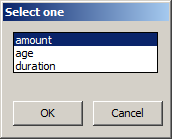
\includegraphics[height=3cm, width=3.712cm]{fig-001-1}  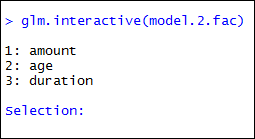
\includegraphics[height=3cm, width=5.504cm]{fig-001-2}
\caption{Initial dialog to select the metric covariate to be displayed.}
\label{fig-001}
\end{figure}

\pagebreak

\item The GUI-panel (see figure~\ref{fig-002}, left) allows the following actions:
\begin{itemize} [leftmargin=0.5cm, rightmargin=0.5cm, label=$\bullet$]
\item The values of the metric covariates can be choosen by sliders. 
\item The type of the termplot to be displayed can be selected in the radiobox \textit{Type}.
\item If factors are present, the level-combinations of the factors to be displayed can be selected in the checkbox \textit{Groups}.
\item Tables of the effects can be printed to the \proglang{R Console} and optionally the actual plot is saved by pushing the button \textit{Snapshot}. The effects are calculated for the covariate constellation chosen by the sliders. 
\end{itemize}

\begin{figure}[ht]
\centering
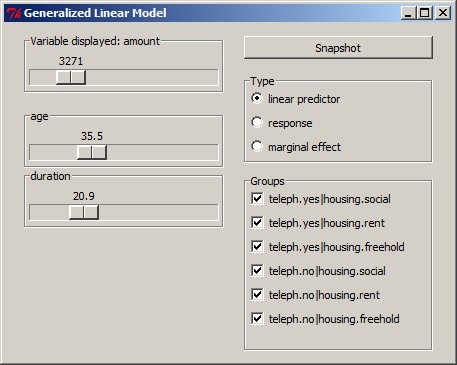
\includegraphics[height=5cm, width=6.26cm]{fig-002-1}   \quad 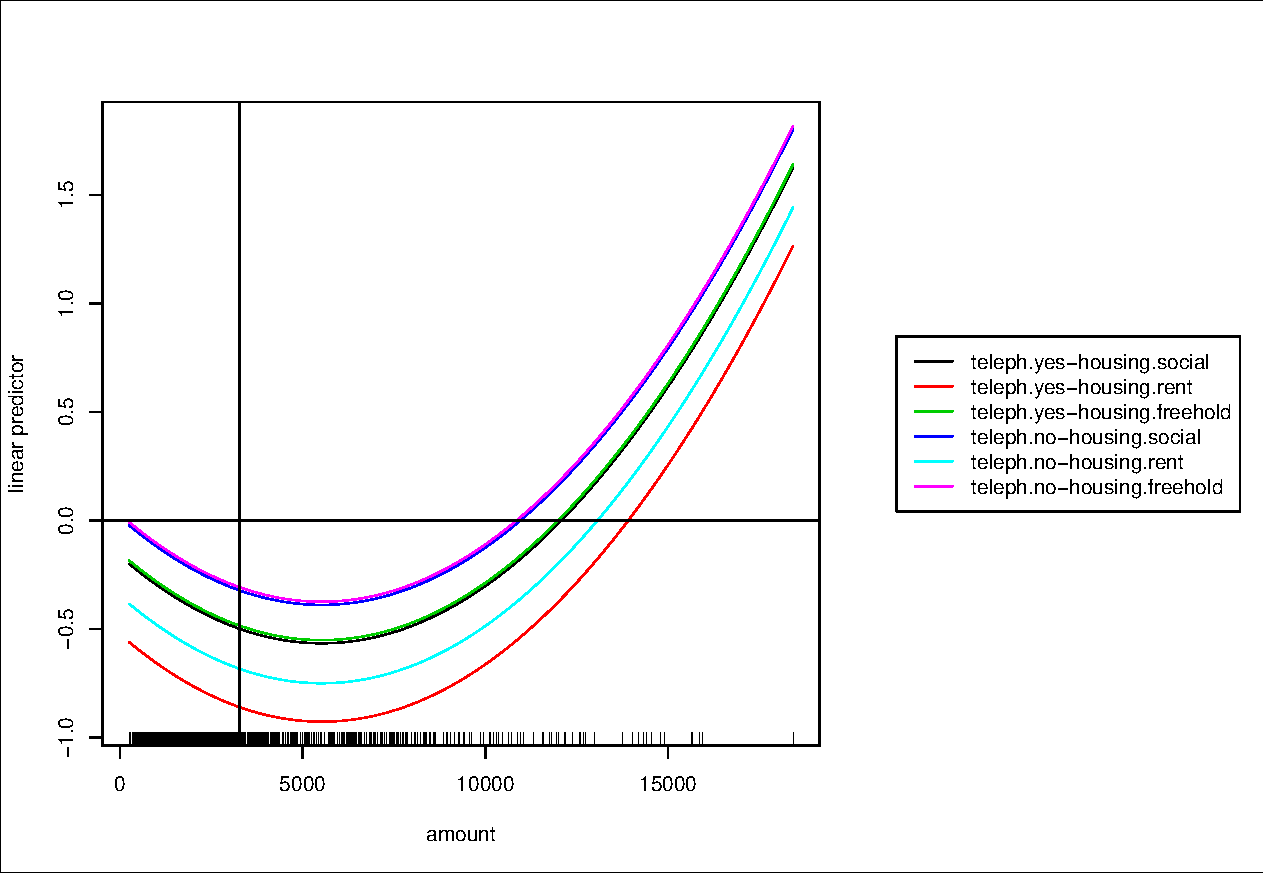
\includegraphics[height=5cm, width=7.233cm]{fig-002-2.pdf}
\caption{GUI-panel and initial termplot (linear predictor) of the selected metric covariate. By default the metric covariates are at their means and all groups are displayed.} \label{fig-002}
\end{figure}
\end{enumerate}

Details on the tables produced by the \textit{Snapshot}-button are explained in section~\ref{sec-output}.
On the right hand side of figure~\ref{fig-002} the initial termplot for the example model is shown.  The plot is optimized for screens and is reduced in size here to fit on the page, therefore the annotations may be hard to read. The termplots are calculated for the range of the selected metric covariate. The top slider controls the value of the selected metric covariate which is used to calculate the output triggered by the \emph{Snapshot}-button. The initial values of the sliders are by default the means of the metric covariates. When the model contains only one metric covariate no selection dialog shows up and no legend is added to the plot. Since the number of resulting groups can become quite large no confidence intervals are implemented yet to keep the plots clear. 

\pagebreak

\section{Visualization of statistical concepts} \label{sec-visualization}
With a focus on the problems pointed out in section~\ref{sec-intro} the usefulness of the function is demonstrated by means of examples in this section. Furthermore the problem of quasi-complete separation is addressed as last example. The plots in this section are customized for printing and the code to reproduce the figures is used as \code{demo} in the package:
%
\begin{Schunk}
\begin{Sinput}
 demo(VignetteFigures, package = "LinRegInteractive", ask = FALSE)
\end{Sinput}
\end{Schunk}
%
Note that 19 PDF-files are stored in the actual working directory by calling the demo.

\subsection{Nonlinear and nonparametric effects in limited dependent variable models}
In the example model of section~\ref{sec-quickstart} the covariate \quotes{amount} is included quadratically. 
Selecting this covariate to be displayed the strong nonlinear effect can be observed in the linear predictors, the responses and the marginal
effects. These  plots are shown in figure~\ref{fig-cd-amount}. The other metric covariates are set to their means and for each of the 6 groups an individual line is plotted. The levels of the factor \quotes{teleph} are represented by shades of red and blue respectively and the levels of the factor \quotes{housing} by a decreasing hue of these colours.  Note that for this particular model specification the lines of the groups \quotes{teleph.yes-housing.social} and \quotes{teleph.yes-housing.freehold} and the lines of the groups \quotes{teleph.no-housing.social} and \quotes{teleph.no-housing.freehold} are almost identical. Therefore the levels \quotes{freehold} and \quotes{social} of the factor \quotes{housing} could be unified for this particular model. Since model specification is not an issue here this will not be discussed further.  

\begin{figure}[ht]
\centering
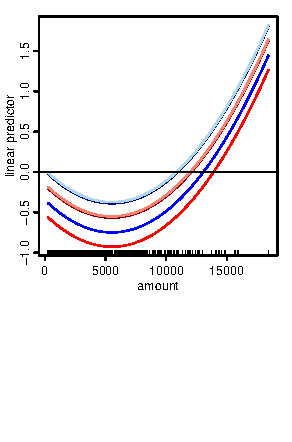
\includegraphics[width=5cm]{cd-amount-link} 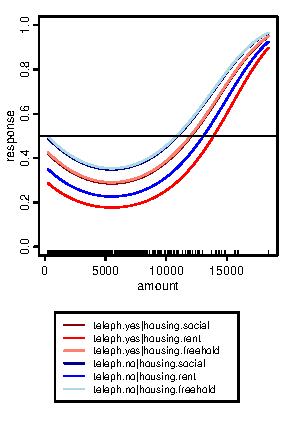
\includegraphics[width=5cm]{cd-amount-resp} 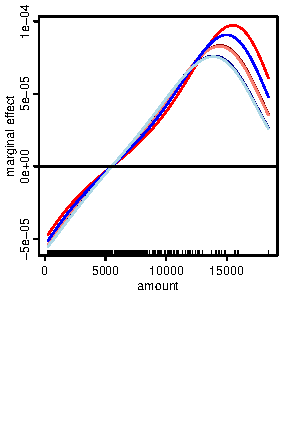
\includegraphics[width=5cm]{cd-amount-marg}
\vspace{-0.75cm}
\caption{Quadratic effects of the metric covariate \quotes{amount} in the linear predictor (left), the response (middle) and the marginal effect (right) in the 6 groups formed by the two factors \quotes{teleph} and \quotes{housing}. The other metric covariates are set to their means.} \label{fig-cd-amount}
\end{figure}

To allow more flexibility in the fit the metric covariate \quotes{amount} can  be included nonparametrically using a spline function. The modified function call is
%
\begin{Schunk}
\begin{Sinput}
 require("splines")
 model.2.fac.npamount <- glm(credit ~ bs(amount) + age + duration*teleph  
     + housing, family = binomial(link="probit"), data = creditdata)
 fxInteractive(model.2.fac.npamount) 
\end{Sinput}
\end{Schunk}
%
The resulting plots are shown in figure~\ref{fig-cd-amount-np} For this plot the other metric covariates are set to their means.  Since the legend is identical to figure~\ref{fig-cd-amount} it is omitted here.

\begin{figure}[ht]
\centering
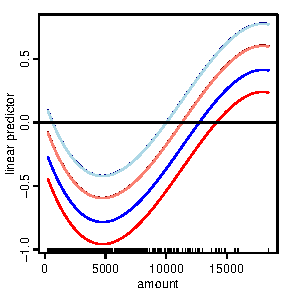
\includegraphics[width=5cm]{cd-amount-np-link} 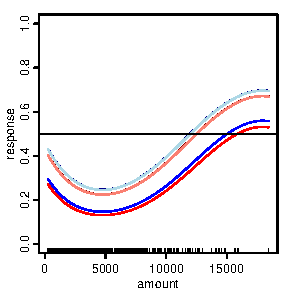
\includegraphics[width=5cm]{cd-amount-np-resp} 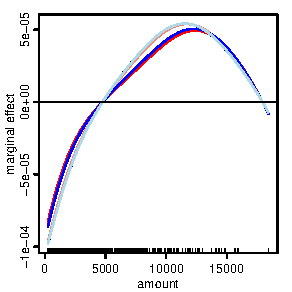
\includegraphics[width=5cm]{cd-amount-np-marg}
\caption{Nonparametric effect of the metric covariate \quotes{amount} in the linear predictor (left), the response (middle) and the marginal effect (right) in the 6 groups formed by the two factors \quotes{teleph} and \quotes{housing}. The other metric covariates are set to their means.} \label{fig-cd-amount-np}
\end{figure}


A generalized additive model can also be employed using the function \code{gam()} from the package \pkg{mgcv} \citep{Wood2014} or from the package \pkg{gam} \citep{Hast2013}:  
\begin{Schunk}
\begin{Sinput}
 require("mgcv") 
 model.2.fac.mgcv <- gam(credit ~ s(amount) + age + duration*teleph + housing,  
     family = binomial(link="probit"), data = creditdata)
 fxInteractive(model.2.fac.mgcv)
\end{Sinput}
\end{Schunk}
%
The resulting plots are shown in figure~\ref{fig-cd-amount-mgcv}, the other metric covariates are set to their means again here.   Since the legend is identical to figure~\ref{fig-cd-amount} it is omitted again. 

\begin{figure}[H]
\centering
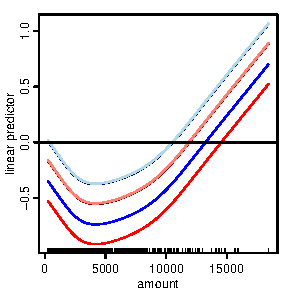
\includegraphics[width=5cm]{cd-amount-mgcv-link} 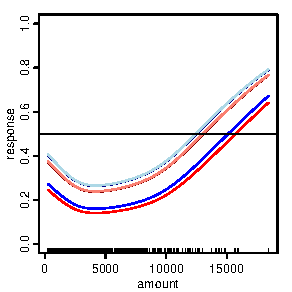
\includegraphics[width=5cm]{cd-amount-mgcv-resp} 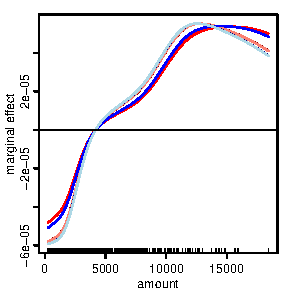
\includegraphics[width=5cm]{cd-amount-mgcv-marg}
\caption{Effect of the metric covariate \quotes{amount} in a generalized additive model in the linear predictor (left), the response (middle) and the marginal effect (right) in the 6 groups formed by the two factors \quotes{teleph} and \quotes{housing}. The other metric covariates are set to their means.} \label{fig-cd-amount-mgcv}
\end{figure}


\subsection{Interaction effects in binary response models}
The mechanics of interaction effects between metric and categorical covariates can easily be observed because in the termplots  every group is represented by an individual line. In the example model of section~\ref{sec-quickstart} there is an interaction between the metric covariate \quotes{duration} and the factor \quotes{teleph}. By choosing \quotes{duration} to be displayed this interaction effect can be observed directly in the linear predictors, the responses and the marginal effects. The corresponding plots are shown in figure \ref{fig-cd-dur-1}, for the plots the other metric covariates are left at their means.  The legend is identical to figure~\ref{fig-cd-amount} and therefore omitted.
\begin{figure}[ht]
\centering
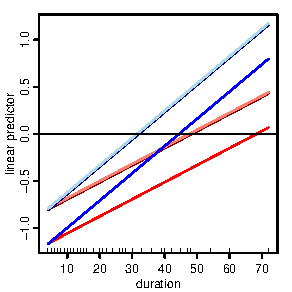
\includegraphics[width=5cm]{cd-dur-link} 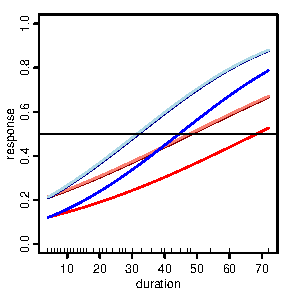
\includegraphics[width=5cm]{cd-dur-resp} 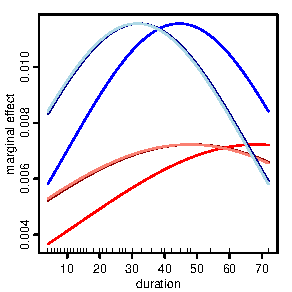
\includegraphics[width=5cm]{cd-dur-marg}
\caption{Direct visualization of the interaction effect between the metric covariate \quotes{duration} and the factor \quotes{teleph} in the linear predictor (left), the response (middle) and the marginal effect (right) in the 6 groups formed by the two factors \quotes{teleph} and \quotes{housing}. The other metric covariates are set to their means.} \label{fig-cd-dur-1}
\end{figure}

Due to the interactive nature of the functions the interaction effect becomes also visible when other covariates are selected to be displayed. The top row of  figure~\ref{fig-cd-age-1} shows the linear predictors, the responses and the marginal effects for the covariate \quotes{age}, the covariate  \quotes{amount} is left at the mean and the covariate \quotes{duration} is set to 12 months.  The legend is identical to figure~\ref{fig-cd-amount} and therefore omitted again. For the plots in the second row the covariate \quotes{duration} is set to 36 months. Due to the interaction effect the red lines are further away from the blue lines compared to the plots in the first row and by this the interaction effect becomes visible indirectly.

\begin{figure}[ht]
\centering
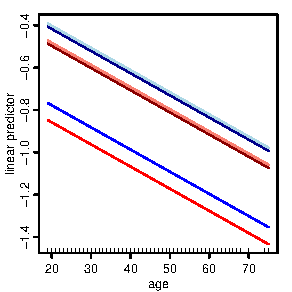
\includegraphics[width=5cm]{cd-age-link-1} 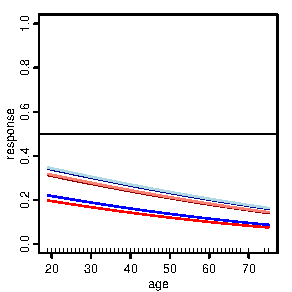
\includegraphics[width=5cm]{cd-age-resp-1} 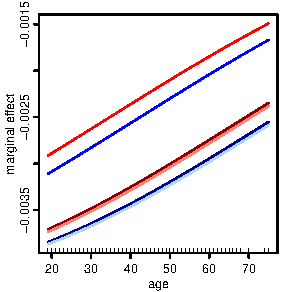
\includegraphics[width=5cm]{cd-age-marg-1}

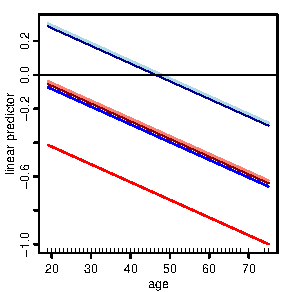
\includegraphics[width=5cm]{cd-age-link-2} 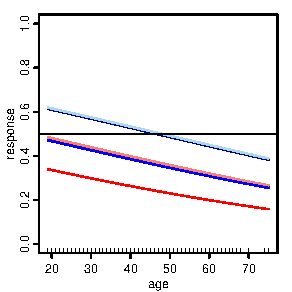
\includegraphics[width=5cm]{cd-age-resp-2} 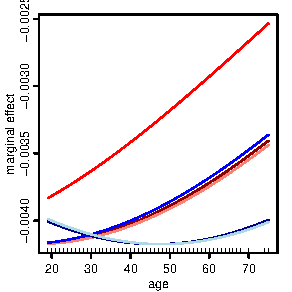
\includegraphics[width=5cm]{cd-age-marg-2}
\caption{Indirect visualization of the interaction effect between the metric covariate \quotes{duration} and the factor \quotes{teleph} in the linear predictor (left), the response (middle) and the marginal effect (right) of the metric covariate \quotes{age} in the 6 groups formed by the two factors \quotes{teleph} and \quotes{housing}. For the figures in the first row the covariate \quotes{duration} is set to 12 months and for the second row to 36 months, the covariate \quotes{amount} is set to the mean.} \label{fig-cd-age-1}
\end{figure}

\subsection{Uncover quasi-complete separation in binary response models}
This issue is discussed in Kleiber, Zeileis (2008), p. 130ff by means of the \code{MurderRates}-data which originate from a study on the deterrent effect of capital punishment in the USA in 1950. The authors uncover the problem of quasi-complete separation by tracing a suspiciously large standard deviation of the coefficient estimate for the dummy variable representing the level \quotes{yes} of the factor \quotes{southern}. It is pointed out that this issue is not uncommon with small data sets but is rarely discussed in textbooks and therefore can easily be overseen. Using \code{fxInteractive()}, choosing for instance the covariate \quotes{income} and selecting the probability termplot (see figure~\ref{fig-qcs}) directly reveals the source of the problem even for inexperienced users: 
%
\begin{Schunk}
\begin{Sinput}
 require("AER")
 data("MurderRates")
 model <- glm(I(executions > 0) ~ time + income + noncauc + lfp + southern, 
     data = MurderRates, family = binomial)
 fxInteractive(model)
\end{Sinput}
\end{Schunk}
%

\begin{figure}[H]
\centering
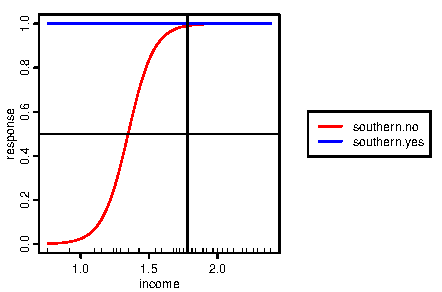
\includegraphics[width=7.5cm]{mr-income-resp}
\caption{The probability termplot of a metric covariate, here \quotes{income}, uncovers the quasi-complete separation in the \code{MurderRates}-data: Observations from the southern states are always predicted as 1.} \label{fig-qcs}
\end{figure}


\section{Details on the text output} \label{sec-output}
The example model from section~\ref{sec-quickstart} is used for illustration in this section with the metric covariates set to their means. The following tables are calculated and printed to the console by clicking the \emph{Snapshot}-button: 
\begin{itemize} [leftmargin=1cm, label=$\bullet$]
\item A summary of the model obtained by \code{summary()} (not shown).
\item Tables of the chosen values of the metric covariates and their ECDF-values (see table~\ref{tab-001}).

\begin{table}[ht]
\centering
\begin{minipage}[c]{8cm}
\begin{CodeChunk}
\small
\begin{CodeOutput}
Selected values of metric covariates
              amount    age duration
value       3271.248 35.542   20.903
ECDF(value)    0.658  0.587    0.554
\end{CodeOutput}
\end{CodeChunk}
\end{minipage}
\caption{Table of the chosen values of the metric covariates and their ECDF-values.} \label{tab-001}
\end{table}

\item In case of limited dependent variable models the table of the link and response function evaluated for the chosen values of the metric covariates in each group (see table~\ref{tab-002}). For other regression models the table of the effects for the chosen values of the metric covariates in each group.

\begin{table}[ht]
\centering
\begin{minipage}[c]{11cm}
\begin{CodeChunk}
\small
\begin{CodeOutput}
Effects in different groups for selected values of metric covariates
                                  link  response
teleph.yes|housing.social   -0.4988935 0.3089272
teleph.yes|housing.rent     -0.8599626 0.1949048
teleph.yes|housing.freehold -0.4843101 0.3140829
teleph.no|housing.social    -0.3219410 0.3737487
teleph.no|housing.rent      -0.6830100 0.2473003
teleph.no|housing.freehold  -0.3073576 0.3792856
\end{CodeOutput}
\end{CodeChunk}
\end{minipage}
\caption{Table of the link and response function for the chosen values of the metric covariates in each group.} \label{tab-002}
\end{table}

\item Table of marginal effects for each metric covariate for the chosen values of the metric covariates 
in each group (see table~\ref{tab-003}). In the case of limited dependent variable models the marginal effects refer to the response function.  The marginal effects are calculated numerically with \code{splinefun()}.

\begin{table}[ht]
\centering
\begin{minipage}[c]{14cm}
\begin{CodeChunk}
\small
\begin{CodeOutput}
Marginal effects in different groups for selected values of metric covariates
                                   amount          age     duration
value                        3.271248e+03 35.542000000 20.903000000
ECDF(value)                  6.580000e-01  0.587000000  0.554000000
teleph.yes|housing.social   -2.092170e-05 -0.003687023  0.006380070
teleph.yes|housing.rent     -1.637027e-05 -0.002884925  0.004992110
teleph.yes|housing.freehold -2.107224e-05 -0.003713551  0.006425975
teleph.no|housing.social    -2.249766e-05 -0.003964754  0.010967026
teleph.no|housing.rent      -1.876481e-05 -0.003306914  0.009147355
teleph.no|housing.freehold  -2.260113e-05 -0.003982988  0.011017466
\end{CodeOutput}
\end{CodeChunk}
\end{minipage}
\caption{Table of marginal effects for each metric covariate for the chosen values of the metric covariates in each group.} \label{tab-003}
\end{table}
\end{itemize}

When the argument \code{latex2console} is set to \code{TRUE} in the call of \code{fxInteractive()} the tables are printed to the console as \LaTeX-code using functions from the package \pkg{xtable}. For the given example the tables in appendix~\ref{sec-appendix-A} show the results.
 A \LaTeX-version of the model summaries is not printed to the console.  For a number of different fitted-model objects the package \pkg{texreg} \citep{Leif2013} provides the functionality to do this.

\section{Details on different aspects of usage} \label{sec-usage}
The arguments explained in this section control different aspects of usage. The explanations in this and the following sections are mostly independent of the class of the fitted-model object provided to \code{fxInteractive()}. Some methods however, for instance the \class{lme}-method for linear mixed-effects models, have additional arguments which are described in the corresponding documentation. The probit model from section~\ref{sec-quickstart} is used as example throughout this section.   

\vspace{-0.3cm}\paragraph{Exact control over metric covariates} 
With the sliders the values of the metric covariates cannot be selected with arbitrary precision. To allow exact control over the values these can be set as initial values for the sliders with the argument \code{initial.values} through a named list. The names in the list must exactly match the variable names:
%
\begin{Schunk}
\begin{Sinput}
 fxInteractive(model.2.fac,
     initial.values = list(amount=5000, duration=24, age=30))
\end{Sinput}
\end{Schunk}
%

If a metric covariate is not explicitly listed the corresponding slider is initialized with the mean (the default). 

\vspace{-0.3cm}\paragraph{Preselect metric covariate, plot type and groups}
To avoid the appearance of the selection menu the name of the metric covariate to be displayed can be preselected:
%
\begin{Schunk}
\begin{Sinput}
 fxInteractive(model.2.fac, preselect.var = "duration")
\end{Sinput}
\end{Schunk}
%
If no metric covariate with the provided name exists the selection menu will pop up instead.

The type of plot to be displayed first can also be specified by the argument \code{preselect.type}. The possible values depend on the class of the fitted-model object, please refer to the documentation of the corresponding method. For the \class{glm}-method for example this must be one of the values \code{"link"} (the default), \code{"response"} or \code{"marginal"}: 
%
\begin{Schunk}
\begin{Sinput}
 fxInteractive(model.2.fac, preselect.type = "response")
\end{Sinput}
\end{Schunk}
%

By default all groups are active in the initial plot. With the argument \code{preselect.groups} the groups  displayed in the initial plot can be specified with a 
numeric index vector. The first three groups are preselected by
%
\begin{Schunk}
\begin{Sinput}
 fxInteractive(model.2.fac, preselect.groups = c(1:3))
\end{Sinput}
\end{Schunk}
%
Preselecting groups is useful if the model contains many factors. In this case the panel usually grows beyond the screen and some groups are not accessible via the GUI-panel any more. The groups are constructed with the function \code{factorCombinations()} which can be used to identify groups of interest. This is illustrated in example B1 in appendix~\ref{sec-app-addexample}. 

The functionality to prespecify the variable, the plot type and certain groups in advance is beneficial when used in conjunction with the argument \code{initial.values} and the automatic save functionality. All taken together, this allows the reproduction of plots without user interaction, see the last example in this section.

\vspace{-0.3cm}\paragraph{Saving plots}
When the argument \code{snapshot.plot} is set to \code{TRUE} the current plot is saved to the working directory when the \emph{Snapshot}-button is pressed. Note that in this case the \proglang{RGui}-window becomes the active window. The type of the plot can be set by the argument \code{graphics.type} which is by default a PDF-file. The allowed file types are platform dependent, please refer to the documentation for possible values.  The advantage to save plots this way instead of using the functionality of the \proglang{RGui} is the handling of the file name.  The file name can be specified in advance  by the argument \code{graphics.filename}. If the argument \code{graphics.numbering} is \code{TRUE} a hyphen followed by a sequential number with 3 digits is added to the file name to avoid that existing plots are overwritten. The path can also be specified within the filename. To save plots of the covariate \quotes{duration} to the directory D:$\backslash$Temp by the \emph{Snapshot}-button one may use
%
\begin{Schunk}
\begin{Sinput}
 fxInteractive(model.2.fac, 
     preselect.var     = "duration",
     snapshot.plot     = TRUE,
     graphics.filename = "D:/Temp/fig-credprobit-duration")
\end{Sinput}
\end{Schunk}
%

When the plot is saved as PDF-file there is sometimes a problem concerning the width of the legend annotations. Depending on the font family and the fontsize in some cases the legend annotations do not fit into the box around the legend in the graphics file even though these do so in the graphics window. A workaround for this is to increase the width of the legend with the argument \code{legend.width.factor}, which is \code{1} by default. If this problem occurs the width of the legend can be increased about 10\% for instance by
%
\begin{Schunk}
\begin{Sinput}
 fxInteractive(model.2.fac, legend.width.factor = 1.1)
\end{Sinput}
\end{Schunk}
%

By setting the argument \code{autosave.plot} to \code{TRUE} the initial plot is saved and the GUI-control is closed immediately after initialization. In conjunction with the 
arguments \code{initial.values}, \code{preselect.var}, \code{preselect.type} and \code{preselect.groups} this can be used to reproduce plots without user interaction. When \code{autosave.plot} is \code{TRUE} the argument \code{graphics.numbering} is set to \code{FALSE} by default. With the following lines the plot of the marginal effects for the example model with 2 factors with a prespecified covariate constellation and a subset of the groups is saved to the actual working directory as PDF-file:
%
\begin{Schunk}
\begin{Sinput}
 fxInteractive(model.2.fac,
     initial.values      = list(amount=5000, duration=24, age=30), 
     preselect.var       = "duration",
     preselect.type      = "marginal",
     preselect.groups    = c(2,3,5,6),
     autosave.plot       = TRUE,
     graphics.filename   = "fig-credprobit-duration-marg",
     legend.width.factor = 1.05)
\end{Sinput}
\end{Schunk}
%

On Windows systems the legend width needs to be increased for the PDF-files to look as expected. The figures of section~\ref{sec-visualization} are created in this reproducible way, the code can be found in the \code{demo} of the package.  

\section{Details on customization} \label{sec-customization}
The appearance of the text output, the plots and the GUI-controls can be customized in many ways.  The arguments for the methods for the different classes of fitted-model object are almost identical. If the arguments vary along the methods this will be mentioned. Two probit models are used for demonstration throughout this section. Firstly the model introduced in section~\ref{sec-quickstart}:
%
\begin{Schunk}
\begin{Sinput}
 data("creditdata")
 model.2.fac <- glm(credit ~ amount + I(amount^2)  + age + duration*teleph
     + housing, family = binomial(link="probit"), data = creditdata)
\end{Sinput}
\end{Schunk}
%
Additionally the following probit model with 3 metric covariates and 3 factors with 2, 3 and 4 levels respectively is also used occasionally:
%
\begin{Schunk}
\begin{Sinput}
 data("creditdata")
 model.3.fac <- glm(credit ~ amount + I(amount^2)  + age + duration*teleph 
     + housing + job, family = binomial(link="probit"), data = creditdata)
\end{Sinput}
\end{Schunk}
%

\subsection{Customize text output} \label{subsec-custom-text}

\vspace{-0.3cm}\paragraph{Separation characters in group names}
Within the group names which are used in the legend and the text output the character separating the factor name and the corresponding factor levels can be set with the argument \code{level.sep} (default to \quotes{.}). The character separating factor-factor level combinations can be set with the argument \code{factor.sep} (default to \quotes{|}). Another reasonable pair of separation characters is for instance
%
\begin{Schunk}
\begin{Sinput}
 fxInteractive(model.2.fac, 
     factor.sep = "-",
     level.sep  = ">")
\end{Sinput}
\end{Schunk}
%

\vspace{-0.3cm}\paragraph{Decimal mark and big mark in \LaTeX-output}
The \LaTeX-output is generated by the functions \code{xtable()} and the corresponding method \code{print.xtable()} from the package \pkg{xtable}. The appearance of the output is controlled by five arguments which are directly passed to these functions. With the arguments \code{xtable.big.mark} and \code{xtable.decimal.mark} the big mark and decimal mark characters can be set.  By default \code{xtable()} uses 2 digits, which can be changed with the argument \code{xtable.digits}.   The overall format of the numbers can be controlled with the argument \code{xtable.display}, please refer to the documentation of \code{xtable()} for possible values. If the horizontal lines should be set with commands from the \LaTeX-package \code{booktabs} the argument \code{xtable.booktabs} must be set to \code{TRUE}.
Changing the \LaTeX-output to the continental European number format with 5 digits and using horizontal lines from the \code{booktabs}-package can be achieved by 
%
\begin{Schunk}
\begin{Sinput}
 fxInteractive(model.2.fac,
     latex2console       = TRUE,
     xtable.big.mark     = ".",
     xtable.decimal.mark = ",",
     xtable.digits       = 5,
     xtable.booktabs     = TRUE)
\end{Sinput}
\end{Schunk}
%

For the \LaTeX-code printed to the console the following preamble (here prepared for German language) for a utf8-encoded TEX-file works well:
\begin{Code}
\documentclass[a4paper]{scrartcl}
\usepackage[T1]{fontenc}
\usepackage[utf8]{inputenx}
\usepackage[ngerman]{babel}
\usepackage[babel,german=quotes]{csquotes}
\usepackage{icomma}
\usepackage{booktabs}
\begin{document}
% copy and paste from R Console
\end{document}
\end{Code}


\subsection{Customize graphic device} \label{subsec-custom-graph}
Many graphical elements can be controlled directly by arguments in the function call. The major appearance of the plots can be controlled by the manipulation of \code{par()}-arguments. If necessary graphical elements can be added to the plots by low-level plotting commands in the \proglang{R Console}. Note that elements added this way are not captured by the autosave functionality described at the end of section~\ref{sec-usage}. The example B2 in appendix~\ref{sec-app-addexample} shows how to save plots without user interaction in this case.

\vspace{-0.3cm}\paragraph{Plot dimensions and pointsize} The dimensions of the graphic device (in centimeters) and the pointsize of plotted text can be set. A more compact plot is for instance obtained by:
%
\begin{Schunk}
\begin{Sinput}
 fxInteractive(model.2.fac, 
     dev.height       = 11,
     dev.width        = 11,
     dev.width.legend = 5,
     dev.pointsize    = 8) 
\end{Sinput}
\end{Schunk}
%

When a legend is added the overall width of the device is \code{dev.width} plus \code{dev.width.legend}. By default a legend is added when at least one factor is used as covariate. For more details on the legend refer to the paragraph \quotes{Legend} in this section.

\vspace{-0.3cm}\paragraph{Vertical limits of the plot}
The vertical limits of the plots are determined automatically by default. If this is not desired the limits can be set manually with the usual  \code{ylim}-argument. For the response function of the example probit model it is reasonable to set the limits to $0$ and $1$: 
%
\begin{Schunk}
\begin{Sinput}
 fxInteractive(model.2.fac,
     preselect.var  = "amount",
     preselect.type = "response",
     ylim           = c(0,1))
\end{Sinput}
\end{Schunk}
%
Note that the vertical limits apply to every kind of plot. Therefore it is usually advisable to fix the limits only if the plots are saved automatically, see section~\ref{sec-usage} for details on this.

\vspace{-0.3cm}\paragraph{Colours, line types and line widths}
The colours, line types and line widths for the lines representing different groups in the plots and the legend can be set directly. For the model with 2 factors the following scheme is suitable:
%
\begin{Schunk}
\begin{Sinput}
 fxInteractive(model.2.fac, 
     col = c(1,"blue",2),
     lwd = rep(c(1,2),each=3))
\end{Sinput}
\end{Schunk}
%
Note that the arguments are recycled if necessary, in this case for the colour. The levels of the factor \quotes{teleph} are represented by the thickness of lines and the levels of the factor \quotes{housing} by the colour.
For the model with 3 factors one may use
%
\begin{Schunk}
\begin{Sinput}
 fxInteractive(model.3.fac,  
     col = rep(c(1,"blue",2), each=4),  
     lty = c(1,2,3,4),
     lwd = rep(c(1,2), each=12),
     dev.width.legend = 8)
\end{Sinput}
\end{Schunk}
%
The levels of the additional factor \quotes{job} are represented by the line type here. The visual discrimination of 4 or more factors will be conceptually hard to achieve. In this case it may be advisable to display only a subset of groups by deselecting the complement groups in the checkbox or by using the argument \code{preselect.groups}. If just  a subset of groups is displayed  it is convenient to set the line formats directly, see the example B3 in appendix~\ref{sec-app-addexample} how to do this.

\vspace{-0.3cm}\paragraph{Title and axis labels}
By default no title is added to the plot, the label for the \emph{x}-axis is the name of the selected covariate and the label for the \emph{y}-axis is the name of the selected plot type. This can be overridden if necessary, for instance with more detailed annotations:
%
\begin{Schunk}
\begin{Sinput}
 fxInteractive(model.2.fac, 
     preselect.var  = "duration",
     preselect.type = "response",
     main           = "Interaction between 'duration' and factor 'teleph'",
     xlab           = "duration (months)",
     ylab           = "probability of credit default")
\end{Sinput}
\end{Schunk}
%
The argument \code{main} is passed to the function \code{title()} which allows to control the vertical position of the headline, the corresponding argument is \code{main.line}. In appendix~\ref{sec-app-addexample} the example B4 shows to customize the title.

\vspace{-0.3cm}\paragraph{Legend}
A legend is added by default when at least one categorical covariate is used. The legend is plotted within an own region with the left and right margin of the legend region set to $0$. The legend frequently needs to be modified since the space required by the legend depends on the number of factors used as covariates, the lengths of the group names,  the physical screen resolution and the size of the \proglang{RGui}-window (if run in  MDI-mode, not relevant for users of \textbf{RStudio}). On the one hand the space for the legend itself can be modified and on the other hand the scaling of the legend. The first solution for the example model with 3 factors is
%
\begin{Schunk}
\begin{Sinput}
 fxInteractive(model.3.fac, dev.width.legend = 8)
\end{Sinput}
\end{Schunk}
%
For the same model reducing the scale to 70\% of the original size also works:
%
\begin{Schunk}
\begin{Sinput}
 fxInteractive(model.3.fac, legend.cex = 0.7)
\end{Sinput}
\end{Schunk}
%
The position of the legend can be modified as well, refer to the documentation of \code{legend()} for details:
%
\begin{Schunk}
\begin{Sinput}
 fxInteractive(model.2.fac, legend.pos = "top")
\end{Sinput}
\end{Schunk}
%
With the argument \code{legend.width.factor} the width of the box around the legend can be manipulated, see the explanations in the paragraph \quotes{Saving plots} in section \ref{sec-usage}.  

When factors are present the legend and the corresponding plot region for it can be completely suppressed by
%
\begin{Schunk}
\begin{Sinput}
 fxInteractive(model.2.fac, legend.add = FALSE)
\end{Sinput}
\end{Schunk}
%
Setting the additional argument \code{legend.space} to \code{TRUE} will create the  corresponding plot region without the legend:
%
\begin{Schunk}
\begin{Sinput}
 fxInteractive(model.2.fac,
     legend.add   = FALSE,
     legend.space = TRUE)
\end{Sinput}
\end{Schunk}
%

This can be useful if different plots are arranged in a document but for only one of the plots a legend should appear. The empty spaces ensure exact alignments and matching plot dimensions in this case. Figure~\ref{fig-cd-amount} in section~\ref{sec-visualization} is an example for this, the code to reproduce the figure can be found in the \code{demo} of the package. To achieve full flexibility for the arrangement of plots in a document the legend can be plotted alone:
%
\begin{Schunk}
\begin{Sinput}
 fxInteractive(model.2.fac, legend.only = TRUE)
\end{Sinput}
\end{Schunk}
%
Since the legend is the only element within the plotting region in this case it is usually reasonable to set the margins to $0$ with the additional argument \code{mar=c(0,0,0,0)}. Note that the width of the graphic device is solely controlled by  \code{dev.width.legend} and in conjunction with \code{dev.height} the overall size of the legend can be set precisely.

\vspace{-0.3cm}\paragraph{Rug plot}
By default a rug representation of the selected metric covariate is added to the southern axis of the plot. The length of the ticks can be controlled with the argument \code{rug.ticksize} which is \code{0.02} by default.  For many observations the rug considerably slows down the rebuild of the plot. Setting \code{rug.ticksize} to \code{0} or \code{NA} removes the rug representation:
%
\begin{Schunk}
\begin{Sinput}
 fxInteractive(model.2.fac, rug.ticksize = NA)
\end{Sinput}
\end{Schunk}
%
The colour of the rug tickmarks can be changed with the argument  \code{rug.col}:
%
\begin{Schunk}
\begin{Sinput}
 fxInteractive(model.2.fac, rug.col = "gray50")
\end{Sinput}
\end{Schunk}
%

If more detailed control over the rug is needed, the rug needs to be suppressed and added  with \code{rug()} from the \proglang{R Console}. The example B2 in section~\ref{sec-app-addexample} shows how to add a customized rug plot with transparent colours.

\vspace{-0.3cm}\paragraph{Vertical and horizontal lines}
To facilitate visual perception a few straight lines are added to the plots by default. A vertical black line shows the actual value of the selected metric covariate. To suppress the vertical line, e.g. for printing the plot, use
%
\begin{Schunk}
\begin{Sinput}
 fxInteractive(model.2.fac, vline.actual = FALSE)
\end{Sinput}
\end{Schunk}
%

By default horizontal black lines are added to the different plots, the vertical positions of the lines can be controlled with the argument \code{pos.hlines}. The argument has to be a numeric vector with the vertical positions of the lines. The length of the vector and the default values depend on the class of the fitted-model object, please refer to the documentation of the corresponding method for details. For the \class{glm}-method the default is for instance the vector \code{c(0,0.5,0)} giving horizontal lines in the plot of the linear predictors at height 0, in the plot of the responses at height 0.5 and in the plot of the marginal effects at height 0. Each line can be suppressed by setting the corresponding value to \code{NA}. For instance suppressing the line for the link function and setting the line in the plot of the response to $0.56$ can be achieved by 
%
\begin{Schunk}
\begin{Sinput}
 fxInteractive(model.2.fac, pos.hlines = c(NA,0.56,0)) 
\end{Sinput}
\end{Schunk}
%
The appearance of the lines (solid black lines) cannot be changed by arguments. To modify this the lines these must be suppressed and added with \code{abline()}-commands afterwards. 

\vspace{-0.3cm}\paragraph{Number of points used for plotting} The effects are plotted for a sequence of equally spaced points over the span of the chosen metric covariate. With the argument \code{n.effects} the number of points can be controlled (default to $100$). If the lines of the effects are not smooth this value can be increased.  

\subsection{Predefining the graphic device} \label{subsec-predefine}
For more control over the appearance of the plots the graphic device can be specified in advance.
Two plot regions which can be accessed with high-level plotting commands are required. The legend is plotted in the first region and the plot itself in the second region to allow the user to add elements to an existing plot with low-level plotting commands. The left and right margin of the legend region are set to $0$. In the following example the legend appears on the left side, the colours are specified via \code{palette()} and the margins as well as the scale of the text are changed. Note that for pointsize $10$ the width of the legend must be increased to achieve that the legend annotations fit into the box of the legend in the PDF-file.   
%
\begin{Schunk}
\begin{Sinput}
 windows(10,7, pointsize = 10)
 layoutmatrix <- matrix(c(1,2,2), 1, 3)
 layout(layoutmatrix)
 palette(c("darkred","red","salmon","darkblue","blue","lightblue"))
 par(cex = 1, mar = c(5,5,2,2)+0.1)
 fxInteractive(model.2.fac,
     preselect.var       = "amount",
     preselect.type      = "response",
     dev.defined         = TRUE,
     ylim                = c(0,1),
     legend.width.factor = 1.1,
     snapshot.plot       = TRUE)
\end{Sinput}
\end{Schunk}
%

\subsection{Customize GUI-controls} \label{subsec-custom-gui}

\vspace{-0.3cm}\paragraph{Size of the GUI-controls} The size of the entire panel is calculated automatically and primarily depends on the number of covariates and groups but also on the screen resolution. Because of this the results from the automatic calculation are sometimes not to 100\% satisfactory, therefore the layout of the panel can be modified by a number of parameters. This can be useful for screens with a low resolution or if the model has a lot of groups. For the latter case the parameters are changed in the following example to save space:
%
\begin{Schunk}
\begin{Sinput}
 fxInteractive(model.3.fac,
     box.type.height           = 90, 
     box.group.character.width = 6, 
     box.group.line.height     = 25, 
     dist.obj.height           = 2)
\end{Sinput}
\end{Schunk}
%

Note that for a large number of groups not every group can be seen in the GUI-panel because the panel grows beyond the screen margin. In former versions of \pkg{rpanel} (< 1.1-3) the entries of the checkbox are squeezed together. Currently there is no way to circumvent this problem. At the moment the only solution is to choose the groups in advance using the argument \code{preselect.groups}, see the paragraph \quotes{Preselect metric covariate, plot type and groups} in section~\ref{sec-usage}.


\vspace{-0.3cm}\paragraph{Annotations of the GUI-controls} The annotations of the GUI-controls can be changed easily, for instance to German: 
%
\begin{Schunk}
\begin{Sinput}
 fxInteractive(model.2.fac,
     panel.title      = "Probit Modell",
     label.button     = "Schnappschuss",
     label.slider.act = "Dargestellte Variable: ",
     label.box.type   = "Typ",
     label.types      = c("Linearer Praediktor", "Wahrscheinlichkeit",
                          "Marginaler Effekt"),
     label.box.groups = "Gruppen")
\end{Sinput}
\end{Schunk}
%
Note that the \code{label.types} for the annotations of the radiobox are used as default annotations for the \emph{y}-axis of the corresponding plots. The length of the character vector and the default entries for this argument depend on the class of the fitted-model object, please refer to the documentation of the corresponding method for details. For the \class{glm}-method for instance a character vector of length~3 to annotate the radiobox choices for the plot of the link functions, the response functions and the marginal effects is required.   



\section{Solving problems with raw data extraction} \label{sec-call-classes}
The internal calculations are based on the prediction method of the fitted-model object and the raw data. Internally it is tried to extract the raw data with \code{get\_all\_vars(model\$terms, model\$data)}. If the fitted-model object lacks a \code{data} slot, it is tried to retrieve the raw data with \code{get\_all\_vars(model\$terms, model\$model)}. For example fitted-model objects of class \class{lm} lack a \code{data} slot and for some formulas the latter extraction method does not work properly, for instance if a covariate is incorporated as spline function via \code{bs()}.  Adding  a \code{data} slot to the fitted-model object afterwards solves this particular problem. This is demonstrated by means of a linear regression model for the rents of apartments in Munich, Germany. The dataset \code{munichrent03} is contained in the package and was originally obtained from the \citet{DataRent2014}. The variables are described in the documentation of the dataset \code{munichrent03}:
%
\begin{Schunk}
\begin{Sinput}
 data("munichrent03")
 require("splines")
 model.rent <- lm(rent ~ bs(yearc) + area*location + upkitchen,
     data=munichrent03)
 model.rent$data <- munichrent03
 fxInteractive(model.rent)
\end{Sinput}
\end{Schunk}
%
Adding a \code{data} slot afterwards may also be helpful if the raw data cannot be extracted for other reasons.

\bibliography{LinRegInteractive}

\newpage

\appendix
\section[Example of LaTeX text output]{Example of \LaTeX ~ text output} \label{sec-appendix-A}
The three tables together with the captions in this section are the text output (see section~\ref{sec-output}) for the model given in section~\ref{sec-quickstart} with the argument \code{latex2console} set to \code{TRUE} and the argument \code{xtable.digits} set to \code{5}.


\begin{table}[ht]
\centering
\begin{tabular}{lrrr}
  \hline
 & amount & age & duration \\ 
  \hline
value & 3.271,24800 & 35,54200 & 20,90300 \\ 
  ECDF(value) & 0,65800 & 0,58700 & 0,55400 \\ 
   \hline
\end{tabular}
\caption{Selected values of metric covariates} 
\label{tab-values}
\end{table}


\begin{table}[ht]
\centering
\begin{tabular}{lrr}
  \hline
 & link & response \\ 
  \hline
teleph.yes$|$housing.social & -0,49889 & 0,30893 \\ 
  teleph.yes$|$housing.rent & -0,85996 & 0,19490 \\ 
  teleph.yes$|$housing.freehold & -0,48431 & 0,31408 \\ 
  teleph.no$|$housing.social & -0,32194 & 0,37375 \\ 
  teleph.no$|$housing.rent & -0,68301 & 0,24730 \\ 
  teleph.no$|$housing.freehold & -0,30736 & 0,37929 \\ 
   \hline
\end{tabular}
\caption{Effects in different groups for selected values of metric covariates} 
\label{tab-effects}
\end{table}


\begin{table}[ht]
\centering
\begin{tabular}{lrrr}
  \hline
 & amount & age & duration \\ 
  \hline
value & 3.271,24800 & 35,54200 & 20,90300 \\ 
  ECDF(value) & 0,65800 & 0,58700 & 0,55400 \\ 
   \hline
teleph.yes$|$housing.social & -0,00002 & -0,00369 & 0,00638 \\ 
  teleph.yes$|$housing.rent & -0,00002 & -0,00288 & 0,00499 \\ 
  teleph.yes$|$housing.freehold & -0,00002 & -0,00371 & 0,00643 \\ 
  teleph.no$|$housing.social & -0,00002 & -0,00396 & 0,01097 \\ 
  teleph.no$|$housing.rent & -0,00002 & -0,00331 & 0,00915 \\ 
  teleph.no$|$housing.freehold & -0,00002 & -0,00398 & 0,01102 \\ 
   \hline
\end{tabular}
\caption{Marginal effects in different groups for selected values of metric covariates} 
\label{tab-marginaleffects}
\end{table}




\section{Additional examples} \label{sec-app-addexample}

\vspace{-0.3cm}\paragraph{Example B1} For models with many groups the GUI-panel grows beyond the screen. The only way to select or deselect the nonvisible groups is to preselect these. In this example only the groups which occur more than 10 times in the data are choosen to be displayed.
%
\begin{Schunk}
\begin{Sinput}
 model.cd.manygroups <- glm(credit ~ amount + I(amount^2) + age 
     + duration*teleph + housing + intuse, family=binomial, data=creditdata)
 factor.combs       <- factorCombinations(creditdata[,c("teleph",
     "housing","intuse")])
 logic.index.groups <- factor.combs$counts > 10
 index.groups       <- seq(along=factor.combs$counts)[logic.index.groups]
 fxInteractive(model.cd.manygroups,
     preselect.var    = "amount",
     preselect.groups = index.groups)
\end{Sinput}
\end{Schunk}
%
\vspace{-0.3cm}\paragraph{Example B2} A customized rug plot with transparent colour is added with the low-level plotting command \code{segments()}, the plot could be saved afterwards in an arbitrary format, here as PDF-file. The function for this is platform dependent, on Windows systems this is \code{savePlot()} and on non-Windows systems the function depends on the desired graphic format.  
%
\begin{Schunk}
\begin{Sinput}
 fxInteractive(model.2.fac, 
     preselect.var  = "amount",
     preselect.type = "response",
     ylim           = c(0,1),
     rug.ticksize   = 0,
     legend.width.factor = 1.1)
 segments(creditdata$amount, par("usr")[3], creditdata$amount, 
     par("fig")[3], col = rgb(0,0,0,0.2))
 # savePlot(filename = "creditdefault-customrug", type = "pdf") # Windows
 # dev.copy2pdf(file = "creditdefault-customrug.pdf") # Non-Windows
\end{Sinput}
\end{Schunk}
%

\vspace{-0.3cm}\paragraph{Example B3}
For models with many groups it is reasonable to display only a subset of the groups and to set the formats directly. In this example the groups in which the credit is used to buy a new car are displayed.
%
\begin{Schunk}
\begin{Sinput}
 model.cd.manygroups <- glm(credit ~ amount + I(amount^2) + age
     + duration*teleph + housing + intuse, family=binomial, data=creditdata)
 index.groups <- c(1,11,21,31,41,51)
 vec.col <- NULL
 vec.col[index.groups] <- c(1:6)
 vec.lty <- NULL
 vec.lty[index.groups] <- rep(c(1,2), each = 3)
 fxInteractive(model.cd.manygroups,
     preselect.var    = "amount",
     preselect.groups = index.groups,
     col              = vec.col,
     lty              = vec.lty)
\end{Sinput}
\end{Schunk}
%

\vspace{-0.3cm}\paragraph{Example B4}
The title of the plot is closer to the surrounding box and set to normal size and plain text:     
%
\begin{Schunk}
\begin{Sinput}
 fxInteractive(model.2.fac, 
     preselect.var  = "duration",
     preselect.type = "link",
     main           = "Interaction between 'duration' and factor 'teleph'",
     main.line      = 0.5,
     cex.main       = 1,
     font.main      = 1)
\end{Sinput}
\end{Schunk}
%

\section{Version history}
\begin{table}[ht]
\centering
\begin{tabular}{lll}
\toprule
Version & Date published & Changes                                           \\ \midrule
0.3-1   & 22.04.2015     & update of contact details \\ \midrule
0.3-0   & 12.11.2014     & switch to the concept of generic functions \\
        &                & LaTeX output is now generated with package \pkg{xtable}\\
        &                & saving plots as PDF should now work on all platforms \\
        &                & automatic file name numbering can be suppressed \\
        &                & minor bugfixes and performance improvements \\
        &                & generic function \texttt{fxInteractive} added  \\
        &                & method for objects of class \texttt{glm} added   \\
        &                & method for objects of class \texttt{lm} added   \\
        &                & method for objects of class \texttt{lme} added   \\
        &                & function \texttt{glm.interactive} removed \\
        &                & function \texttt{lm.interactive} removed \\
        &                & function \texttt{factor.combinations()} renamed  \\
        &                & \quad  to \texttt{factorCombinations()} \\
        &                & argument  \texttt{ylim} added \\
        &                & argument  \texttt{main.line} added \\ 
        &                & arguments \texttt{pos.hline.xxx} replaced by argument \texttt{pos.hlines}   \\
        &                & argument  \texttt{graphics.extension} renamed to \texttt{graphics.type} \\
        &                & argument  \texttt{graphics.numbering} added \\
        &                & argument  \texttt{decimal.mark} renamed to \texttt{xtable.decimal.mark} \\
        &                & argument  \texttt{big.mark} renamed to \texttt{xtable.big.mark} \\
        &                & argument  \texttt{xtable.digits} added \\
        &                & argument  \texttt{xtable.display} added \\
        &                & argument  \texttt{xtable.booktabs} added \\ \midrule
0.2-2   & 08.09.2014     & vignette revised \\\midrule
0.2-1   & 26.08.2014     & argument \texttt{preselect.groups} added          \\
        &                & argument \texttt{select.all.groups.begin removed} \\
        &                & problem with flickering plot solved         \\
        &                & no restrictions for the names of factors/factor levels any more \\ \midrule
0.1-3   & 18.08.2014     & first published version                           \\ \bottomrule
\end{tabular} 
\end{table}

\end{document}
